\documentclass{vgtc} 
\usepackage[brazilian]{babel}
\usepackage[utf8]{inputenc}
\usepackage{mathptmx}
\usepackage{graphicx}
\usepackage{times}

\usepackage{xurl}


\onlineid{0}
\vgtccategory{Research}

\title{Título do PF 1}


\author{Nome Aluno$^{1}$\thanks{e-mail: email@somewhere.com} %
\and Nome Professor$^{2}$}
\affiliation{\scriptsize $^{1}$Universidade do Vale do Rio dos Sinos, Jogos Digitais, Brasil\\
$^{2}$Universidade do Vale do Rio dos Sinos, Jogos Digitais, Brasil}

%% A teaser figure can be included as follows:
\teaser{
   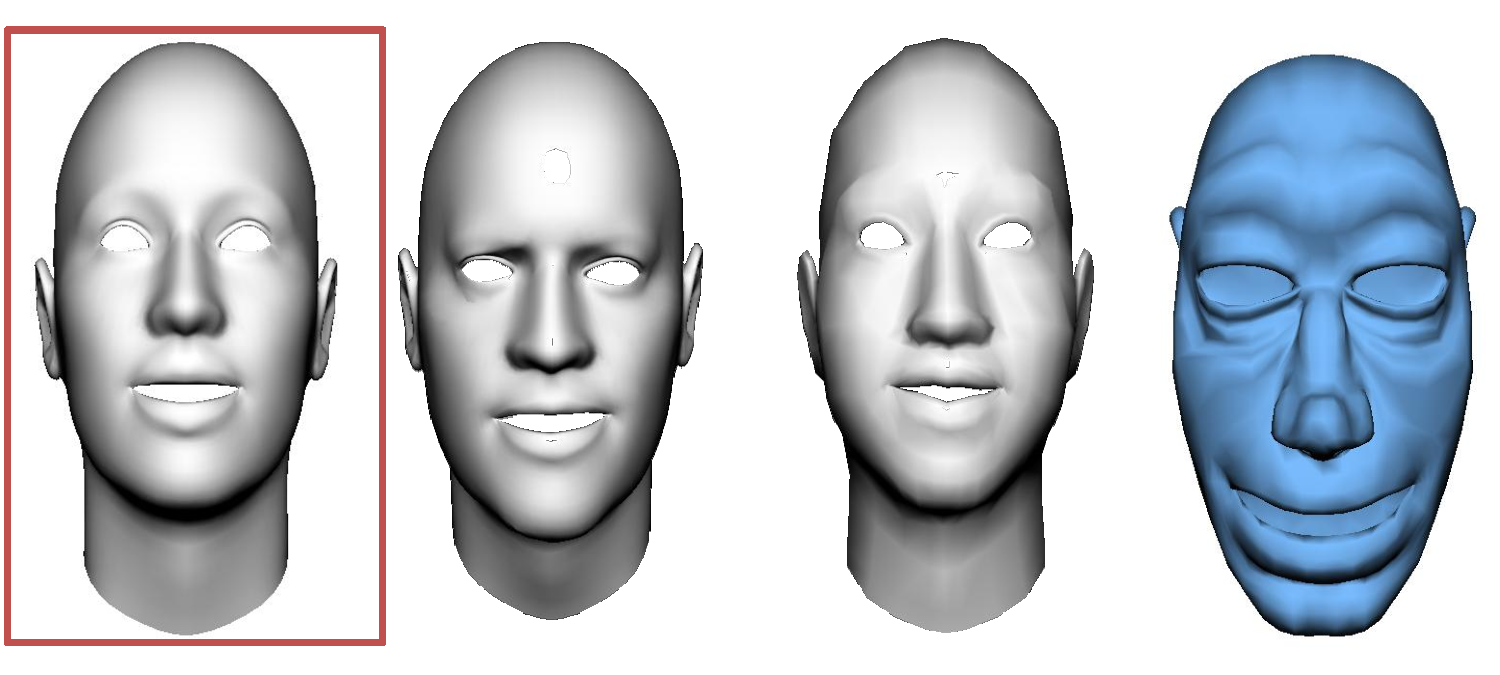
\includegraphics[width=0.5\linewidth]{figs/openSmile.pdf}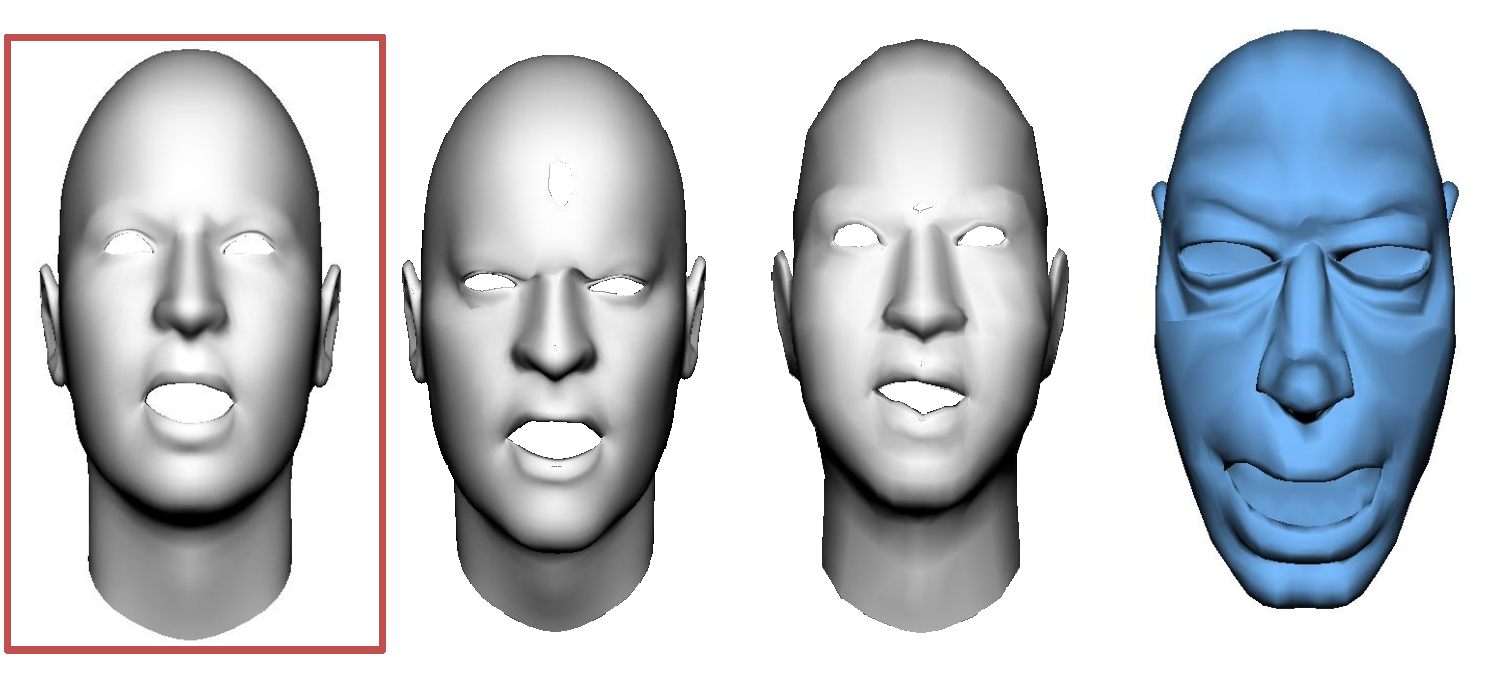
\includegraphics[width=0.5\linewidth]{figs/angryFace.pdf} 
  \caption{A figura de \emph{teaser} é opcional, e em geral usamos ela para mostrar alguns resultados visuais mais relevantes do trabalho (para "vender o peixe" visualmente).}
  \label{figura:teaser}
}


\abstract{O resumo de um artigo deve conter, em poucas palavras: uma frase que resume o objetivo principal, uma ou duas frases que explicam qual foi a metodologia e/ou principais técnicas utilizadas para alcançar este objetivo, como o resultado obtido foi avaliado e o resumo das principais conclusões/discussões obtidas pela avaliação dos resultados.

\smallskip
%pelo menos 3 palavras-chave relacionadas ao trabalho (pense como se fossem as hashtags para que seu trabalho seja encontrado)
\noindent \textbf{Palavras-chave:} Jogos Digitais; Animação Facial; \emph{Rigging} Facial; Transferência de Expressões.
} 

%%%%%%%%%%%%%%%%%%%%%%%%%%%%%%%%%%%%%%%%%%%%%%%%%%%%%%
%% INICIO DO ARTIGO
%%%%%%%%%%%%%%%%%%%%%%%%%%%%%%%%%%%%%%%%%%%%%%%%%%%%%%

\begin{document}

\firstsection{Introdução}
\label{secao:introducao}
\maketitle

%Se quiser colocar outra seção basta criar um novo arquivo .tex e usar o \input para inclui-lo
Na seção introdutória do trabalho, você deve escrever, no mínimo, as seguintes coisas a respeito do trabalho, cada uma delas ocupando de 1 a 3 parágrafos (preferivelmente) 

\subsection{Motivação}
\label{secao:motivacao}
Nestes primeiros parágrafos do artigo, você descreve o que motiva o desenvolvimento do trabalho (motivos sólidos baseados na pesquisa de referências, como deficiência no mercado a ser suprida, área pouco explorada, grande demanda do mercado por determinada tecnologia ou inovação).  

\subsection{Objetivo Geral}
\label{secao:objetivo_geral}
Aqui você deixa bem claro o objetivo principal do trabalho -- o que foi desenvolvido (ou no caso de PF1, o que está em desenvolvimento): ``Este trabalho apresenta o desenvolvimento do jogo \emph{Fellowsheep Adventures in Creepyland}, um jogo de simulação de ovelhas que possuem o poder de alterar as expressões faciais de seus pastores, que pensam ter controle sobre elas." 

Também deve ser feita uma rápida contextualização (conexão entre a motivação e o objetivo). ``Neste contexto, o jogo explora elementos de jogos Simulação como o Happy Farm\footnote{My Invention, 2019} e Sim City 2000\footnote{Maxis, 1999} combinados com o gênero de Aventura e utilizando no game design conceitos de expressões faciais propostos por Ekman~\cite{Ekman:1978}".

Exemplo de referência à Seção \ref{secao:objetivos_especificos}.

\subsection{Objetivos Específicos}
\label{secao:objetivos_especificos}
Lorem ipsum dolor sit amet, consectetuer adipiscing elit, sed diam nonummy nibh euismod tincidunt ut laoreet dolore magna aliquam erat volutpat. Ut wisi enim ad minim veniam, quis nostrud exercitation ullamcorper suscipit lobortis nisl ut aliquip ex ea commodo consequat. Duis autem vel eum iriure dolor in hendrerit in vulpu-tate velit esse molestie consequat, vel illum dolore eu feugiat nulla facilisis at vero eros et accumsan et iusto odio dignissim qui blan-dit praesent luptatum zzril delenit augue duis dolore te feugait nulla facilisi.

\subsection{Estrutura do Artigo}
\label{secao:estrutura_do_artigo}
    \item O artigo está organizado da seguinte maneira: a Seção~\ref{secao:analise_pesquisa_de_mercado} apresenta um levantamento de jogos relacionados e questões de mercado relacionadas com o jogo em desenvolvimento. Logo após, a Seção~\ref{secao:jogo} apresenta (...), seguida da Seção~\ref{secao:desenvolvimento} que descreve em detalhes as decisões projetuais e tecnolõgicas mais importantes no processo de desenvolvimento do jogo. Em seguida, são apresentados resultados das avaliações realizadas na Seção~\ref{secao:testes}, a análise de resultados na Seção~\ref{secao:analise_de_resultados} e por último, são apresentadas considerações e trabalhos futuros na Seção~\ref{secao:consideracoes_finais}.
\section{ANÁLISE DE MERCADO}
\label{secao:analise_pesquisa_de_mercado}
Lorem ipsum dolor sit amet, consectetuer adipiscing elit, sed diam nonummy nibh euismod tincidunt ut laoreet dolore magna aliquam erat volutpat. Ut wisi enim ad minim veniam, quis nostrud exercitation ullamcorper suscipit lobortis nisl ut aliquip ex ea commodo consequat. Duis autem vel eum iriure dolor in hendrerit in vulpu-tate velit esse molestie consequat, vel illum dolore eu feugiat nulla facilisis at vero eros et accumsan et iusto odio dignissim qui blan-dit praesent luptatum zzril delenit augue duis dolore te feugait nulla facilisi.
Exemplo de referência à Figura \ref{figura:exemplo}.

\begin{figure}[htb]
  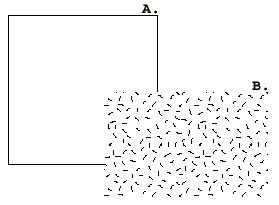
\includegraphics[width=0.8\columnwidth]{figure.jpg}
  \centering
  \caption{Exemplo de figura. Fonte: Autor.}
  \label{figura:exemplo}
\end{figure}

\subsection{Concorrentes}
\label{secao:concorrentes}
Lorem ipsum dolor sit amet, consectetuer adipiscing elit, sed diam nonummy nibh euismod tincidunt ut laoreet dolore magna aliquam erat volutpat. Ut wisi enim ad minim veniam, quis nostrud exercitation ullamcorper suscipit lobortis nisl ut aliquip ex ea commodo consequat. Duis autem vel eum iriure dolor in hendrerit in vulpu-tate velit esse molestie consequat, vel illum dolore eu feugiat nulla facilisis at vero eros et accumsan et iusto odio dignissim qui blan-dit praesent luptatum zzril delenit augue duis dolore te feugait nulla facilisi.
Exemplo de citação de Tweet \cite{stacey2011}

\subsection{Inspirações}
\label{secao:inspiracoes}
Lorem ipsum dolor sit amet, consectetuer adipiscing elit, sed diam nonummy nibh euismod tincidunt ut laoreet dolore magna aliquam erat volutpat. Ut wisi enim ad minim veniam, quis nostrud exercitation ullamcorper suscipit lobortis nisl ut aliquip ex ea commodo consequat. Duis autem vel eum iriure dolor in hendrerit in vulpu-tate velit esse molestie consequat, vel illum dolore eu feugiat nulla facilisis at vero eros et accumsan et iusto odio dignissim qui blan-dit praesent luptatum zzril delenit augue duis dolore te feugait nulla facilisi.

\subsection{Monetização}
\label{secao:monetizacao}
Lorem ipsum dolor sit amet, consectetuer adipiscing elit, sed diam nonummy nibh euismod tincidunt ut laoreet dolore magna aliquam erat volutpat. Ut wisi enim ad minim veniam, quis nostrud exercitation ullamcorper suscipit lobortis nisl ut aliquip ex ea commodo consequat. Duis autem vel eum iriure dolor in hendrerit in vulpu-tate velit esse molestie consequat, vel illum dolore eu feugiat nulla facilisis at vero eros et accumsan et iusto odio dignissim qui blan-dit praesent luptatum zzril delenit augue duis dolore te feugait nulla facilisi.

\begin{quote}
	Lorem ipsum dolor sit amet, consectetur adipiscing elit. Curabitur at maximus neque. Sed molestie sodales malesuada. Nunc laoreet aliquet sagittis. Proin ornare congue volutpat. Morbi elit orci, elementum eget gravida et, ultrices eget leo. Donec eleifend, orci pulvinar sagittis consequat, erat nibh imperdiet tortor, id tempus urna nulla id leo. Donec consectetur mi vel orci pellentesque auctor.  \cite[p. 7]{notes2002}.
\end{quote}


\section{Jogo}
\label{secao:jogo}
Lorem ipsum dolor sit amet, consectetuer adipiscing elit, sed diam nonummy nibh euismod tincidunt ut laoreet dolore magna aliquam erat volutpat. Ut wisi enim ad minim veniam, quis nostrud exercitation ullamcorper suscipit lobortis nisl ut aliquip ex ea commodo consequat. Duis autem vel eum iriure dolor in hendrerit in vulpu-tate velit esse molestie consequat, vel illum dolore eu feugiat nulla facilisis at vero eros et accumsan et iusto odio dignissim qui blan-dit praesent luptatum zzril delenit augue duis dolore te feugait nulla facilisi.

\subsection{Roteiro}
\label{secao:roteiro}
Lorem ipsum dolor sit amet, consectetuer adipiscing elit, sed diam nonummy nibh euismod tincidunt ut laoreet dolore magna aliquam erat volutpat. Ut wisi enim ad minim veniam, quis nostrud exercitation ullamcorper suscipit lobortis nisl ut aliquip ex ea commodo consequat. Duis autem vel eum iriure dolor in hendrerit in vulpu-tate velit esse molestie consequat, vel illum dolore eu feugiat nulla facilisis at vero eros et accumsan et iusto odio dignissim qui blan-dit praesent luptatum zzril delenit augue duis dolore te feugait nulla facilisi.

\subsection{\textit{Gameplay}}
\label{secao:gameplay}
Lorem ipsum dolor sit amet, consectetuer adipiscing elit, sed diam nonummy nibh euismod tincidunt ut laoreet dolore magna aliquam erat volutpat. Ut wisi enim ad minim veniam, quis nostrud exercitation ullamcorper suscipit lobortis nisl ut aliquip ex ea commodo consequat. Duis autem vel eum iriure dolor in hendrerit in vulpu-tate velit esse molestie consequat, vel illum dolore eu feugiat nulla facilisis at vero eros et accumsan et iusto odio dignissim qui blan-dit praesent luptatum zzril delenit augue duis dolore te feugait nulla facilisi.

\subsection{Elementos de \textit{Gameplay}}
\label{secao:elementos_de_gameplay}
Lorem ipsum dolor sit amet, consectetuer adipiscing elit, sed diam nonummy nibh euismod tincidunt ut laoreet dolore magna aliquam erat volutpat. Ut wisi enim ad minim veniam, quis nostrud exercitation ullamcorper suscipit lobortis nisl ut aliquip ex ea commodo consequat. Duis autem vel eum iriure dolor in hendrerit in vulpu-tate velit esse molestie consequat, vel illum dolore eu feugiat nulla facilisis at vero eros et accumsan et iusto odio dignissim qui blan-dit praesent luptatum zzril delenit augue duis dolore te feugait nulla facilisi.

\subsubsection{Jogador}
\label{secao:jogador}
Lorem ipsum dolor sit amet, consectetuer adipiscing elit, sed diam nonummy nibh euismod tincidunt ut laoreet dolore magna aliquam erat volutpat. Ut wisi enim ad minim veniam, quis nostrud exercitation ullamcorper suscipit lobortis nisl ut aliquip ex ea commodo consequat. Duis autem vel eum iriure dolor in hendrerit in vulpu-tate velit esse molestie consequat, vel illum dolore eu feugiat nulla facilisis at vero eros et accumsan et iusto odio dignissim qui blan-dit praesent luptatum zzril delenit augue duis dolore te feugait nulla facilisi.

\subsubsection{Personagens}
\label{secao:personagens}
Lorem ipsum dolor sit amet, consectetuer adipiscing elit, sed diam nonummy nibh euismod tincidunt ut laoreet dolore magna aliquam erat volutpat. Ut wisi enim ad minim veniam, quis nostrud exercitation ullamcorper suscipit lobortis nisl ut aliquip ex ea commodo consequat. Duis autem vel eum iriure dolor in hendrerit in vulpu-tate velit esse molestie consequat, vel illum dolore eu feugiat nulla facilisis at vero eros et accumsan et iusto odio dignissim qui blan-dit praesent luptatum zzril delenit augue duis dolore te feugait nulla facilisi.

\subsubsection{Obstáculos}
\label{secao:obstaculos}
Lorem ipsum dolor sit amet, consectetuer adipiscing elit, sed diam nonummy nibh euismod tincidunt ut laoreet dolore magna aliquam erat volutpat. Ut wisi enim ad minim veniam, quis nostrud exercitation ullamcorper suscipit lobortis nisl ut aliquip ex ea commodo consequat. Duis autem vel eum iriure dolor in hendrerit in vulpu-tate velit esse molestie consequat, vel illum dolore eu feugiat nulla facilisis at vero eros et accumsan et iusto odio dignissim qui blan-dit praesent luptatum zzril delenit augue duis dolore te feugait nulla facilisi.

\subsubsection{Fases}
\label{secao:fases}
Lorem ipsum dolor sit amet, consectetuer adipiscing elit, sed diam nonummy nibh euismod tincidunt ut laoreet dolore magna aliquam erat volutpat. Ut wisi enim ad minim veniam, quis nostrud exercitation ullamcorper suscipit lobortis nisl ut aliquip ex ea commodo consequat. Duis autem vel eum iriure dolor in hendrerit in vulpu-tate velit esse molestie consequat, vel illum dolore eu feugiat nulla facilisis at vero eros et accumsan et iusto odio dignissim qui blan-dit praesent luptatum zzril delenit augue duis dolore te feugait nulla facilisi.

\section{Jogabilidade e Mecânicas}
\label{secao:jogabilidade_mecanicas}
Lorem ipsum dolor sit amet, consectetuer adipiscing elit, sed diam nonummy nibh euismod tincidunt ut laoreet dolore magna aliquam erat volutpat. Ut wisi enim ad minim veniam, quis nostrud exercitation ullamcorper suscipit lobortis nisl ut aliquip ex ea commodo consequat. Duis autem vel eum iriure dolor in hendrerit in vulpu-tate velit esse molestie consequat, vel illum dolore eu feugiat nulla facilisis at vero eros et accumsan et iusto odio dignissim qui blan-dit praesent luptatum zzril delenit augue duis dolore te feugait nulla facilisi.

\subsection{Arte}
\label{secao:arte}
Lorem ipsum dolor sit amet, consectetuer adipiscing elit, sed diam nonummy nibh euismod tincidunt ut laoreet dolore magna aliquam erat volutpat. Ut wisi enim ad minim veniam, quis nostrud exercitation ullamcorper suscipit lobortis nisl ut aliquip ex ea commodo consequat. Duis autem vel eum iriure dolor in hendrerit in vulpu-tate velit esse molestie consequat, vel illum dolore eu feugiat nulla facilisis at vero eros et accumsan et iusto odio dignissim qui blan-dit praesent luptatum zzril delenit augue duis dolore te feugait nulla facilisi.

\subsection{Trilha Sonora}
\label{secao:trilha_sonora}
Lorem ipsum dolor sit amet, consectetuer adipiscing elit, sed diam nonummy nibh euismod tincidunt ut laoreet dolore magna aliquam erat volutpat. Ut wisi enim ad minim veniam, quis nostrud exercitation ullamcorper suscipit lobortis nisl ut aliquip ex ea commodo consequat. Duis autem vel eum iriure dolor in hendrerit in vulpu-tate velit esse molestie consequat, vel illum dolore eu feugiat nulla facilisis at vero eros et accumsan et iusto odio dignissim qui blan-dit praesent luptatum zzril delenit augue duis dolore te feugait nulla facilisi.

\subsection{Efeitos Sonoros}
\label{secao:efeitos_sonoros}
Lorem ipsum dolor sit amet, consectetuer adipiscing elit, sed diam nonummy nibh euismod tincidunt ut laoreet dolore magna aliquam erat volutpat. Ut wisi enim ad minim veniam, quis nostrud exercitation ullamcorper suscipit lobortis nisl ut aliquip ex ea commodo consequat. Duis autem vel eum iriure dolor in hendrerit in vulpu-tate velit esse molestie consequat, vel illum dolore eu feugiat nulla facilisis at vero eros et accumsan et iusto odio dignissim qui blan-dit praesent luptatum zzril delenit augue duis dolore te feugait nulla facilisi.

\subsection{Interface Gráfica}
\label{secao:interface_grafica}
Lorem ipsum dolor sit amet, consectetuer adipiscing elit, sed diam nonummy nibh euismod tincidunt ut laoreet dolore magna aliquam erat volutpat. Ut wisi enim ad minim veniam, quis nostrud exercitation ullamcorper suscipit lobortis nisl ut aliquip ex ea commodo consequat. Duis autem vel eum iriure dolor in hendrerit in vulpu-tate velit esse molestie consequat, vel illum dolore eu feugiat nulla facilisis at vero eros et accumsan et iusto odio dignissim qui blan-dit praesent luptatum zzril delenit augue duis dolore te feugait nulla facilisi.
\section{Desenvolvimento}
\label{secao:desenvolvimento}
Lorem ipsum dolor sit amet, consectetuer adipiscing elit, sed diam nonummy nibh euismod tincidunt ut laoreet dolore magna aliquam erat volutpat. Ut wisi enim ad minim veniam, quis nostrud exercitation ullamcorper suscipit lobortis nisl ut aliquip ex ea commodo consequat. Duis autem vel eum iriure dolor in hendrerit in vulpu-tate velit esse molestie consequat, vel illum dolore eu feugiat nulla facilisis at vero eros et accumsan et iusto odio dignissim qui blan-dit praesent luptatum zzril delenit augue duis dolore te feugait nulla facilisi.


\begin{equation}
 \sum_{j=1}^{z} j = \frac{z(z+1)}{2}
\end{equation}

Exemplo de citação de um artigo\cite{Nielson:1991:TAD}.

\subsection{Metodologia de Desenvolvimento}
\label{secao:metodologia_de_desenvolvimento}
Explicar brevemente o ciclo de desenvolvimento com as principais etapas (preferencialmente uma metodologia de game design já estabelecida)

\subsection{Tecnologias Utilizadas}
\label{secao:tecnologias_utilizadas}
Explicar brevemente como foi feita a implementação dos principais elementos do jogo (efeitos - shaders, técnicas de animação, técnicas de IA, Física, UI, etc).


\subsection{\textit{Assets}/Recursos Utilizados}
\label{secao:assets_recursos_utilizados}
Lorem ipsum dolor sit amet, consectetuer adipiscing elit, sed diam nonummy nibh euismod tincidunt ut laoreet dolore magna aliquam erat volutpat. Ut wisi enim ad minim veniam, quis nostrud exercitation ullamcorper suscipit lobortis nisl ut aliquip ex ea commodo consequat. Duis autem vel eum iriure dolor in hendrerit in vulpu-tate velit esse molestie consequat, vel illum dolore eu feugiat nulla facilisis at vero eros et accumsan et iusto odio dignissim qui blan-dit praesent luptatum zzril delenit augue duis dolore te feugait nulla facilisi.

\subsection{Otimizações}
\label{secao:otimizacoes}
Lorem ipsum dolor sit amet, consectetuer adipiscing elit, sed diam nonummy nibh euismod tincidunt ut laoreet dolore magna aliquam erat volutpat. Ut wisi enim ad minim veniam, quis nostrud exercitation ullamcorper suscipit lobortis nisl ut aliquip ex ea commodo consequat. Duis autem vel eum iriure dolor in hendrerit in vulpu-tate velit esse molestie consequat, vel illum dolore eu feugiat nulla facilisis at vero eros et accumsan et iusto odio dignissim qui blan-dit praesent luptatum zzril delenit augue duis dolore te feugait nulla facilisi.

\section{Testes}
\label{secao:testes}
Descrever os testes aplicados, tais como:
\begin{enumerate}
    \item Testes de viabilidade
    \item Testes com usuários
    \item Ferramentas de avaliação (Google ou Unity Analytics, por exemplo)
    
\end{enumerate}

Descrever os testes realizados, o número e perfil dos usuários que testaram (sexo, idade, etc)

Testes qualitativos: mostrar gráficos da avaliação dos usuários

Testes quantitativos: se possível, levanter algumas estatísticas


\subsection{Testes de Implementação}
\label{secao:testes_de_implementacao}
Lorem ipsum dolor sit amet, consectetuer adipiscing elit, sed diam nonummy nibh euismod tincidunt ut laoreet dolore magna aliquam erat volutpat. Ut wisi enim ad minim veniam, quis nostrud exercitation ullamcorper suscipit lobortis nisl ut aliquip ex ea commodo consequat. Duis autem vel eum iriure dolor in hendrerit in vulpu-tate velit esse molestie consequat, vel illum dolore eu feugiat nulla facilisis at vero eros et accumsan et iusto odio dignissim qui blan-dit praesent luptatum zzril delenit augue duis dolore te feugait nulla facilisi.

\subsection{Testes de Usabilidade}
\label{secao:testes_de_usabilidade}
Lorem ipsum dolor sit amet, consectetuer adipiscing elit, sed diam nonummy nibh euismod tincidunt ut laoreet dolore magna aliquam erat volutpat. Ut wisi enim ad minim veniam, quis nostrud exercitation ullamcorper suscipit lobortis nisl ut aliquip ex ea commodo consequat. Duis autem vel eum iriure dolor in hendrerit in vulpu-tate velit esse molestie consequat, vel illum dolore eu feugiat nulla facilisis at vero eros et accumsan et iusto odio dignissim qui blan-dit praesent luptatum zzril delenit augue duis dolore te feugait nulla facilisi.

\subsection{\textit{Testes de Jogabilidade}}
\label{secao:Playtest}
Lorem ipsum dolor sit amet, consectetuer adipiscing elit, sed diam nonummy nibh euismod tincidunt ut laoreet dolore magna aliquam erat volutpat. Ut wisi enim ad minim veniam, quis nostrud exercitation ullamcorper suscipit lobortis nisl ut aliquip ex ea commodo consequat. Duis autem vel eum iriure dolor in hendrerit in vulpu-tate velit esse molestie consequat, vel illum dolore eu feugiat nulla facilisis at vero eros et accumsan et iusto odio dignissim qui blan-dit praesent luptatum zzril delenit augue duis dolore te feugait nulla facilisi.

\section{Análise de Resultados}
\label{secao:analise_de_resultados}
Lorem ipsum dolor sit amet, consectetuer adipiscing elit, sed diam nonummy nibh euismod tincidunt ut laoreet dolore magna aliquam erat volutpat. Ut wisi enim ad minim veniam, quis nostrud exercitation ullamcorper suscipit lobortis nisl ut aliquip ex ea commodo consequat. Duis autem vel eum iriure dolor in hendrerit in vulpu-tate velit esse molestie consequat, vel illum dolore eu feugiat nulla facilisis at vero eros et accumsan et iusto odio dignissim qui blan-dit praesent luptatum zzril delenit augue duis dolore te feugait nulla facilisi.

\section{Considerações Finais}
\label{secao:consideracoes_finais}
Mais ou menos 3 a 5 parágrafos discutindo os resultados, procurando levantar e, se possível, justificar:

\begin{itemize}
    \item Pontos fortes 
    \item Pontos a serem melhorados
\end{itemize}

\subsection{Trabalhos Futuros}
Identificar e discutir trabalhos futuros (próximas etapas).

Melhorias

Publicação, monetização
% conference papers do not normally have an appendix


% use section* for acknowledgement
\section*{Agradecimentos}

\begin{itemize}
    \item Consultores ou professores que não tenham participado de forma ativa nos projetos (deram
algumas sugestões técnicas, mas não trabalharam em conjunto – como auxiliar na escrita, por exemplo)\footnote{nesta hora vale o bom senso, principalmente se o artigo for submetido para conferências e/ou journals. Se for submeter, converse com seu professor sobre as autorias.}
    \item Colaboradores: pessoas que contribuíram com assets, pessoas que contribuíram tecnicamente
    \item Programas que financiaram/patrocinaram o trabalho (se houver)
    \item Pessoas que colaboraram nas avaliações/testes (não precisa nomear todas) 
    \item Pessoas que deram suporte emocional/afetivo (pais, amigos, conjuges etc)
\end{itemize}

%Suporte a citação de tweets
\bibliographystyle{utphystw}

% Se não quiser usar tweets
%\bibliographystyle{abbrv}
\bibliography{template}
\end{document}
